

%\documentclass[10pt,iop]{emulateapj}
\documentclass[preprint]{aastex}

\usepackage{url}
\usepackage{multirow}
\usepackage{amsmath}
\usepackage{xcolor}
%\citestyle{aa}

%\bibliographystyle{apj_w_etal}

\newcommand{\etal}{{et al.\/}}
\newcommand{\Prob}{\mathtt{P}}
\newcommand{\logL}{\log\mathcal{L}}
\newcommand{\unit}[1]{\footnotesize #1}
\newcommand{\PAPER}{\mathrm{PAPER}}
\bibliographystyle{apj_w_etal}

\newcommand{\Nconf}{31}
\newcommand{\Nsrc}{32}
\definecolor{orange}{RGB}{255,127,0}

	% End definitions

%\slugcomment{DRAFT: \today}

\shorttitle{EoR time}
\shortauthors{Jacobs et al.}

\begin{document}


\title{Multi-redshift limits on the 21cm power spectrum from PAPER}
\author{
Daniel C. Jacobs\altaffilmark{1},
Aaron R. Parsons\altaffilmark{2,8},
James E. Aguirre\altaffilmark{3},
Zaki Ali\altaffilmark{2},
Judd Bowman\altaffilmark{1},
Richard F. Bradley\altaffilmark{4,5,6},
Chris L.  Carilli\altaffilmark{7},
David R. DeBoer\altaffilmark{8},
Matthew R. Dexter\altaffilmark{8},
Nicole E. Gugliucci\altaffilmark{5},
Pat Klima\altaffilmark{5},
Adrian Liu\altaffilmark{2,11},
Dave H. E. MacMahon\altaffilmark{8}
Jason R. Manley\altaffilmark{9},
David F. Moore\altaffilmark{3},
Jonathan C. Pober\altaffilmark{2},
Irina I. Stefan\altaffilmark{10},
William P. Walbrugh\altaffilmark{9}}

\altaffiltext{1}{School of Earth and Space Exploration, Arizona State U., Tempe, AZ}
\altaffiltext{2}{Astronomy Dept., U. California, Berkeley, CA}
\altaffiltext{3}{Dept. of Physics and Astronomy, U. Pennsylvania, Philadelphia, PA}
\altaffiltext{4}{Dept. of Electrical and Computer Engineering, U. Virginia, Charlottesville, VA}
\altaffiltext{5}{National Radio Astronomy Obs., Charlottesville, VA}
\altaffiltext{6}{Dept. of Astronomy, U. Virginia, Charlottesville, VA}
\altaffiltext{7}{National Radio Astronomy Obs., Socorro, NM}
\altaffiltext{8}{Radio Astronomy Lab., U. California, Berkeley, CA}
\altaffiltext{9}{Square Kilometer Array, South Africa Project, Cape Town, South Africa}
\altaffiltext{10}{Cavendish Lab., Cambridge, UK}
\altaffiltext{11}{Berkeley Center for Cosmological Physics, UC Berkeley, Berkeley,
CA}

\begin{abstract}
We present new observations from the Donald C. Backer Precision Array for Probing the Epoch of Reionization (PAPER) telescope which place new lower limits on the HI power spectrum over the redshift range of $7.5<z<10.5$, extending previously published single redshift results to cover the full range accessible to the instrument. The epoch of reionization power spectrum is expected to evolve strongly with redshift, and it is this variation with cosmic history that will allow us to begin to place constraints on the physics of reionization.  The primary obstacle to this goal are bright foregrounds and the attendant systematics associated with high dynamic range measurements. Here we use foreground removal techniques that take advantage of the large instrumental bandwidth to make a high dynamic range estimate of smooth foreground power.  Power spectra at different points across the spectrum reveal the variable efficacy of this subtraction.  Noise limited measurements of $\Delta^2$ at $k=$0.2hMpc$^{-1}$ reach as low as 29mK at redshift 7.5.  Most spectra demonstrate a robust foreground removal of foreground signals to the thermal noise limit, leaving systematics on the scale of the noise. We find that in the case of the highest redshift power spectrum, foregrounds begin to dominate over the noise, reflecting the increased difficulty in filtering foregrounds near the edge of the instrumental band.
\end{abstract}

\keywords{reionization}


\section{Introduction}
The Epoch of Reionization, when the first stars ionized the pervasive cosmological Hydrogen in the last global phase change is predicted to be observable in highly redshifted 21 cm radiation.  The Donald C. Backer Precision Array for Probing the Epoch of Reionization (PAPER, \cite{Parsons:2010p6757})\footnote{\url{eor.berkeley.edu}} is a low frequency radio interferometer experiment dedicated to opening this window on the universe.  Challenges include foregrounds which are brighter by several orders of magnitude and long integration times necessitated by the limited collecting areas of first generation instruments. Direct observation of hydrogen before and during re-ionization is predicted to deliver a wealth of cosmological and astrophysical data, including the nature of the first stellar objects and the timing and rate of galaxy formation, reviews on the physics of reionization as well as theory about the nature of foregrounds maybe be found in \citet{Furlanetto:2006p2267,Morales:2010p8093,Pritchard:2012p9555}.  

Telescopes seeking to measure this signal include the Giant Metre-wave Radio Telescope (GMRT; \cite{Paciga:2013p9943}), the Low Frequency Array (LOFAR; \cite{Yatawatta:2013p9699}) and the Murchison Widefield Array (MWA; \cite{Bowman:2013p9950} and \cite{Tingay:2013p9022}). PAPER is located in the Karoo desert at the site of the South African portion of the future Square Kilometer Array. PAPER has doubled in size on a yearly basis since 2009, making observations with each array.  


Here we report on deep integrations made with a 32 element array in 2011, first described in \cite{Parsons:2013p9876}, hereafter P14.  In P14 we described in detail our reduction method and gave deep new limits on the HI power spectrum in the presence of bright foregrounds at redshift 7.68 using 92 nights (1800 hours) of data.  The epoch of reionization signal is expected to evolve strongly with redshift, and it is this variation with cosmic history that will allow us to begin to place constraints on the physics of reionization \cite{Pritchard:2008p8123,Pober:2014p10390}.  Therefore, while a detection of the 21 cm signal at even a single frequency would be a tremendous breakthrough, analysis techniques must be developed to capitalize on the wide bandwidths of the current generations of high redshift 21cm telescopes.  Using the same data as P14, this paper presents new power spectrum upper limits covering the redshift range $10.5>z>7.2$.  In section  \ref{sec:obs_meth} we summarize the observation and reduction methodology, we present the new upper limits in \ref{sec:results}, and in \ref{sec:conclusion} we offer conclusions and discussion of future work.



%
%This signal is though to be the richest data set on the sky!  Many telescopes are searching for the power spectral signature of 
%HI.  Coarsely, models of 21cm emission can be distilled into two parameters. The redshift at which point the universe was 50\% ionized ($z_i$) and the transition time from mostly neutral to mostly ionized $dz$. Thus full coverage of the spectrum is essential.


%This paper extends the result ARP2013a to cover the redshift range XXX.

\section{Observations}
\label{sec:observations}
The work here follows the same basic procedure and uses the same underlying data set as P14. Here we provide a quick summary and refer the reader to \cite{Parsons:2013p9876} for a more in depth discussion.  A general overview of the PAPER system can be found in \cite{Parsons:2010p6757}, calibration of the primary beam in \cite{Pober:2012p8800}, and imaging results in \cite{Jacobs:2011p8438,Jacobs:2013p10014,Stefan:2013p9926}.  Sensitivity analysis described in \cite{Parsons:2012p9028} revealed that for the low gain elements employed by PAPER, a highly redundant ``grid'' type arrangement offers a significant sensitivity boost.  In most interferometers each baseline samples a different mode of the power spectrum; the ideal case for reconstructing images.  In a grid, there are many samples of each of these cosmological modes which can be averaged to a high sensitivity before being combined with other different $k$ modes.  The PAPER South Africa 32 antenna deployment (PSA32) was arranged in a 4x8 grid with a column spacing of 30m and a row spacing of 4m.  In our analysis, as in P14, we include only the three shortest types of spacings where the reionization power is expected to be brightest. This selection includes those between adjacent columns and within at least one row of each other, a selection containing 70 $\sim$30m-long baselines.

Observations spanning the band between 100 to 200-MHz ($13.1>z>6.1$) were recorded at a resolution of 48kHz and 10.7s  beginning Dec 7, 2011 and ending March 19, 2012 (with some down-time for maintenance) after a total of 92 nights or 1800 hours.  Within this set we included observations in the LST range 1h - 9h where the sky dominated system temperature is at a minimum.  Note that this LST range is slightly shorter than in P14 which extended to LST of 12 hours. These last three hours were found to contribute minimally to increasing sensitivity while being dominated by bright galactic foreground emission and so have been excluded here.




\section{Reduction}
\label{sec:obs_meth}
Here we summarize our data reduction steps, for detailed descriptions see section 3 of P14.

In several stages throughout the analysis process we take a 2D Fourier transform of the visibility spectra $V(\nu,t)$ into ``delay/fringe rate'' space where delay is the Fourier dual to frequency and similarly fringe-rate for time.  In this space, smooth spectrum sources are physically localized to delays shorter than the light travel time length of the baseline (e.g. sources at the horizon, in the direction of the baseline vector) and fringe rates shorter than the sidereal rate.  In this Fourier space, sources are highly localized with deviations from a flat spectrum manifesting as a slight dispersion. The spectrum sampling function, which is uneven due to flagging of interference takes the form of a convolution by a point-spread-function in the same way an imperfect sampling of the uv plane gives rise to the angular psf of an interferometer.  To account for this, we use a CLEAN like, iterative, peak-finder and subtraction algorithm which is limited to finding peaks within the physically allowable ranges.

The data analysis pipeline essentially consists of iterative application of the delay/fringe rate transform process, with an ever tightening allowable number of modes, interleaved with stages of averaging (time, frequency, night), before finally computing a power spectrum.  This final step takes advantage of the redundant baselines to make an unbiased power spectrum estimate by cross-multiplying identical baselines and then averaging the power spectrum modes.  Here we are also using the approximation that over short ($\delta z < \sim 0.5$) the delay spectrum is a good approximation of a sample of the 3D power spectrum \citep{Parsons:2012p8896}.  Thus as we step through the various iterations of delay spectrum we have the ability to isolate and subtract foregrounds in the native domain of the measured power spectrum. Note that isolation of foregrounds to a region below line-of-site $k_\parallel$s that increases with baseline length is also the much discussed "wedge" \cite{Liu:2014p10462,Liu:2014p10463,Pober:2013p9942,Morales:2012p8790,Vedantham:2012p10297,Datta:2010p8781}. As we only have a single length of baseline the wedge becomes a narrow slice indeed.  The details of each application of the delay/fringe-rate transform will be laid out the following sections as we provide a brief walk-through of the processing pipeline. 


\subsection{Selection of Redshift Bins}
The redshift bins for which we have computed power spectra --shown in Figure \ref{fig:bins}-- have been selected from the available bandwidth using two criteria: minimizing covariance between redshifts and avoiding missing data. We minimize covariance between adjacent redshift bins by limiting overlap of each bin to the spectrum at the outer half of the bin channel range which, as will be described in section \ref{sec:power_spectrum} is significantly down-weighted by the use of a Blackman-Harris window.   The power spectrum method developed in P14 leverages the redundant baselines to estimate non-sky covariance and project out these contaminated modes. This inversion is particularly sensitive to missing data -the inverse of the covariance is not defined- so we also select only channels that have no missing data over the entire sidereal period (see the dotted line in \ref{fig:bins}).  With these constraints we arrive at the redshifts 10.3, 8.5,7.9 and 7.5.  For the purposes of comparison with P14 we also include the redshift 7.86 bin.

The spectral width of the redshift bins is dictated by the competing needs of sensitivity and foreground reduction which both benefit from wider bandwidths and the likely rate of reionization evolution which is thought to be close to $\Delta z \approx 0.5$, which to a good approximation is given for bandwidth $B$ and frequency $f$ as $\Delta z=1421 B/f^2\approx 0.5$. To balance these two competing constraints we choose a single spectral bandwidth of 20Mhz, weighted by a Blackman-Harris window for an effective width of 10Mhz, or $\Delta z=0.5$ at $z=7.45$ ranging up to a $\Delta z = 0.86$ at redshift 10.3.




\subsection{Initial Averaging}
  First, the raw data are down-selected to just the 70 30m long baselines described in Section \ref{sec:observations}.  %I know this isn't technically true, but I think its important that the downselect is obvious up front.
   The visibilities are then compressed in the frequency and time directions by removing delay modes above the horizon and highest frequency fringe rates for a 300m baseline.  This filtering\footnote{See Appendix A of P14} is done in tandem with a radio frequency interference (RFI) flagging step, using the residuals which have had bright sky-like signals removed to flag 4$\sigma$ deviations before feeding the flags back into another iteration of the compression step. This mitigates the effects of bright, narrow band, interference  being scattered into Reionization delay modes and results in a time and frequency bin of length 39.6s and width 492.61kHz. 
  This process reduces the data volume by a factor of $\sim$20, or roughly an order of magnitude improvement on traditional time and frequency averaging which in this array would be limited to ~100kHz and 10s to avoid averaging away fringes.
  
\subsection{Calibration}
We model the gain as a per-antenna amplitude and a phase slope -physically a single time delay- and single low order polynomial passband for all antennae.  Because the array samples correlations redundantly, the relative calibration between antennae is numerically overdetermined and tractable as a linear algebra problem \cite{Liu:2010p10391}.  As described in P14, we compute the ratio between redundant baselines, fit for a gain and phase slope and then algebraically solve for a per-antenna solution.  Using this method we have avoided calibrating each channel independently to preserve as much frequency variation as possible.   These solutions vary little over the three month observing period, exhibiting less than 1\% rms variation. A single solution derived for for the Dec 7 data set is used for the entire observing run. Time and frequency variation of redundant solutions is explored in detail in Zheng et al (in prep).  

Relative calibration is all that is necessary to form a power spectrum, however to set the flux scale, we must form a beam on a bright known point source.  By itself, the redundant solution is completely independent of any sky model. The redundant solution contains two free delay parameters and an overall amplitude scale. We fit the two delay parameters to a model of Pictor A, Fornax A, and the Crab Nebula during a time when the sky is dominated by these three sources while marginalizing over the unknown\footnote{Unknown in the sense of a joint uncertainty in source flux and primary beam pattern.} apparent flux ratio between the three sources. With the delays in place we are now able form a beam on Pictor A and (for each channel) set the overall amplitude to the calibration value of 381Jy found in \cite{jacobs:2013b}.
  
  
 \begin{figure}
\centering
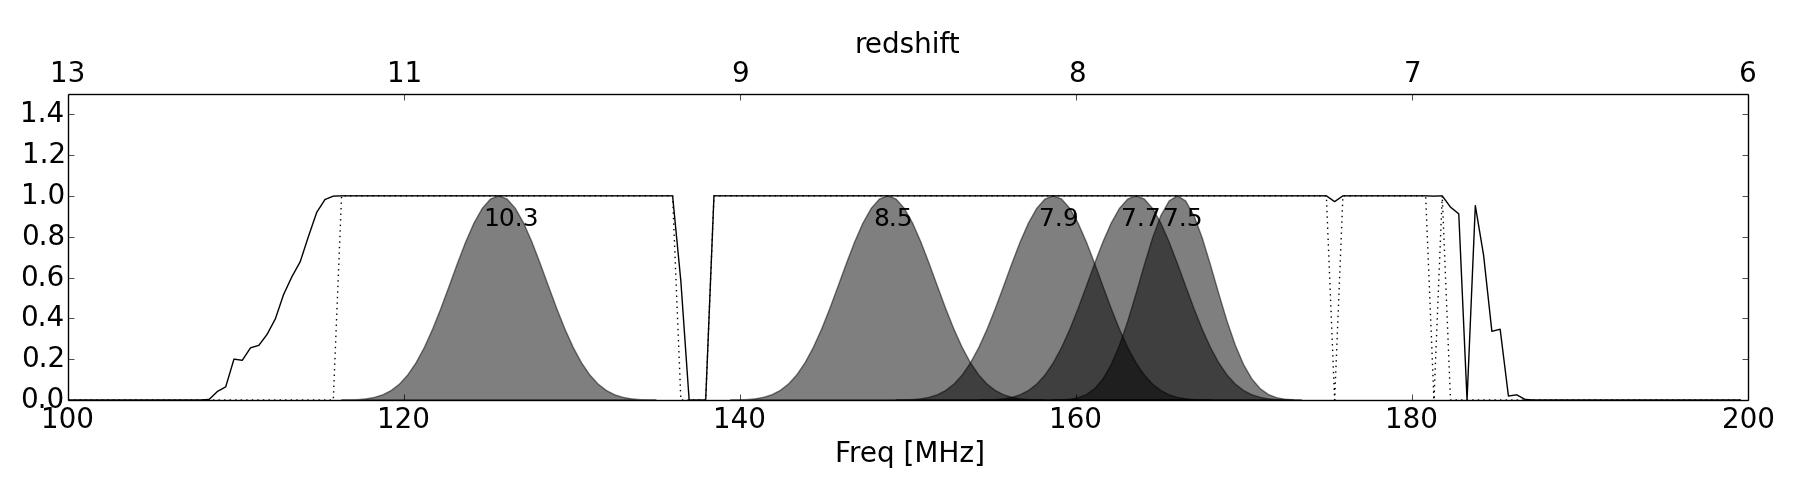
\includegraphics[width=\textwidth]{figures/psa32_flagging_zbins.png}
\caption{\label{fig:bins} The average amount of data remaining after interference flagging over the 3 month period between Dec 2011 and March 2012 (black line) is quite high.  Redshift bins (in grey, redshift center indicated with text label) are chosen to include spectral channels with uniform weight, i.e. no missing channels while maximizing coverage over the band.  Redshift 7.68 is included for comparison with P14.  Channels with no missing data are indicated by the dotted line. Each redshift bin is 20 MHz wide, but weighted by a Blackman-Harris window function which heavily down-weights the outer 10MHz for a Noise Equivalent Bandwidth of 10MHz.  The interference is almost exclusively dominated by two features: ORBCOMM satellites at 137MHz and an unidentified intermittent line emitter at 175MHz. The roll off at 115MHz is due the rising noise at low frequencies being incorrectly flagged as interference.  }
\end{figure} 
%The success of the remainder of the processing stages hinges on the spectral stability of the data, which can easily be assessed by comparing redundant baselines. In figure XXX we see the rms of the ratios between redundant calibrations, before and after the calibration has been applied.  
\begin{figure}
\centering
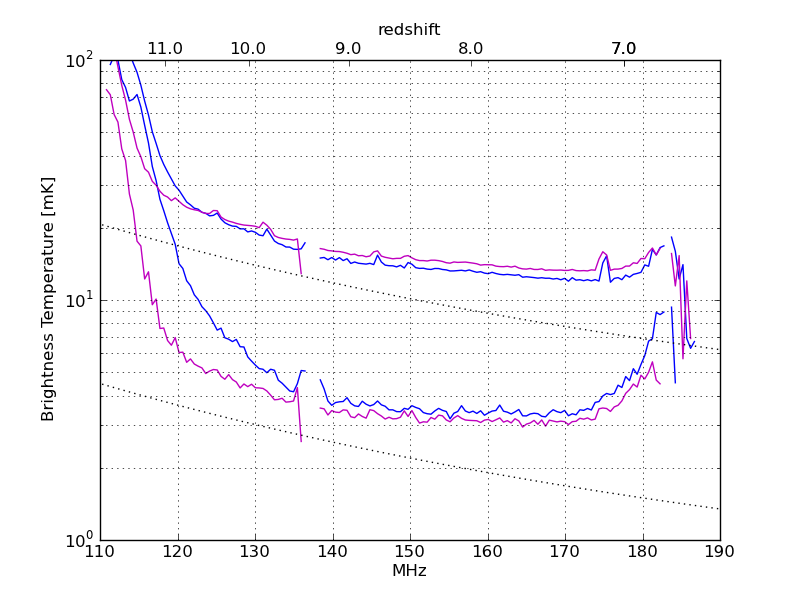
\includegraphics[width=\textwidth]{figures/psa32_trms_with_and_without_fr_filtering_z.png}
\caption{\label{fig:noise} Root mean square (rms) noise before and after integrating to 10 minute LST bins (top and bottom sets of curves) indicating the rising significance of foregrounds as we take the last deep integration step. Noise is estimated by differencing adjacent frequencies (magenta) and between redundant baselines (blue), compared with an estimate of the theoretical noise level (dotted). The top three lines show noise after filtering foregrounds and binning into 40s long sidereal bins.  At this noise level the frequency and baseline differences are roughly similar, both demonstrate the same small bumps of increased noise due to interference flagging and are consistent with noise over much of the band.  The bottom three lines show the noise level after integrating up to the maximum fringe rate of 776s. The step between the top and bottom sets is the last coherent integration with noise largely decreasing by the expected factor $\sqrt{776/40}$ except in the difference between baselines (blue) which demonstrates a clear excess at all frequencies, particularly above redshift 10. With this last large jump in sensitivity we are now seeing the slight dominance of baseline covariance over the spectral derivative rms. }
\end{figure}

\subsection{Foreground Filtering and Night Averaging}
Foregrounds are filtered from the calibrated data by removing all bright delay components with light travel times less then the baseline length. Where during the previous compression step a liberal horizon of 300m (1800ns, much longer than the 30 meter baselines under study)  was used to calculate the window size, we now choose a window corresponding to the 30m baselines under study.  The broadband delay spectrum model is iteratively built then subtracted from the data leaving residuals which we carry into the next stage. Next, a four hour long running mean is subtracted. This removes excess correlation due to cross-talk in the analog signal chain. The residuals are then flagged once more for RFI before the 92 nights of data are averaged into 36.4 second long local sidereal time (LST) bins, which as PAPER is a drift scanning instrument, are equivalent to bins in Right Ascension/ Declination.  During averaging we found that some LST bins were dominated by a small number of exceedingly bright samples lying well outside the rest of the gaussian distributed data. To compensate we filter the 10\% brightest sources in each bin.  The source of these outliers is not known,  a likely possibility is instability in the analog signal chain stimulated by weather or bright interference, a circumstance that has since been observed in later seasons. 


Though the frequency and repeated nightly observations have been averaged to their maximum extent, at 40s integrations the time axis has yet to be fully exploited.  Sky-like fringes on a 30m baseline rotate much slower than 40 seconds.  Performing a final fringe-rate filter, limiting to fringe-rates expected on a 30m baseline (down from 300m in the last iteration), we arrive at a data-set averaged to 789s, the maximum possible while still maintaining fringe coherence.    The root mean square of the residual signal (seen in Figure \ref{fig:noise}) at the end of this process is close to the 3mK level expected given the total integration time.  

%This step is the first point at which signal loss could occur. To measure the loss we add white noise into the data at a level sufficient to double the system temperature (to make it easily detectable on the output), subtract  and then measure the fractional difference post filtration. We recover XXX\% of the injected signal.

%delay transform, covariance projection (lossless, and lossy), bin and bootstrap average,
\subsection{Power Spectrum}
\label{sec:power_spectrum}
The output of the forgoing is a single calibrated and foreground filtered sidereal night. The power spectrum is estimated in the delay spectrum of  a 10MHz bandwidth range centered on the redshift of interest. To preserve the isolation of any foregrounds which remain, we increase the spectral range by 5MHz on each side and multiply by a Blackman-Harris window thus providing a much higher dynamic range delay spectrum point spread function. 

This leaves us with 40 delay samples on each of 70 baselines which are divided into three redundant groups. Within these groups we compute the  correlation between each mode.  The cross correlation of the same delay modes between different redundant baselines provides our estimate of the power spectrum.  Cross correlation between different delay modes provides our measure of systematic bias.  Sky-like correlations should be identical between all redundant baselines to within the level of the noise. In practice some correlations deviate significantly from the median.  These are removed by iteratively dividing the covariance into a model of systematics and a model of sky-like emission and then projecting out large residual modes. This is done by dividing the baselines into different groups such that all cross-multiplications are done without introducing noise bias.  For more see Appendix of C of P14.

The residual correlations are all samples of the power spectrum. To estimate the final power spectrum and its uncertainty we compute the mean and variance of many random randomly-selected subsamples, sampling the dimensions: sidereal time, redundant baseline pair, and delay sign\footnote{As visibilities are complex, both the positive and negative delays  carry  information. Physically the two signs correspond to the two halves of the sky.}



\begin{figure}
\centering
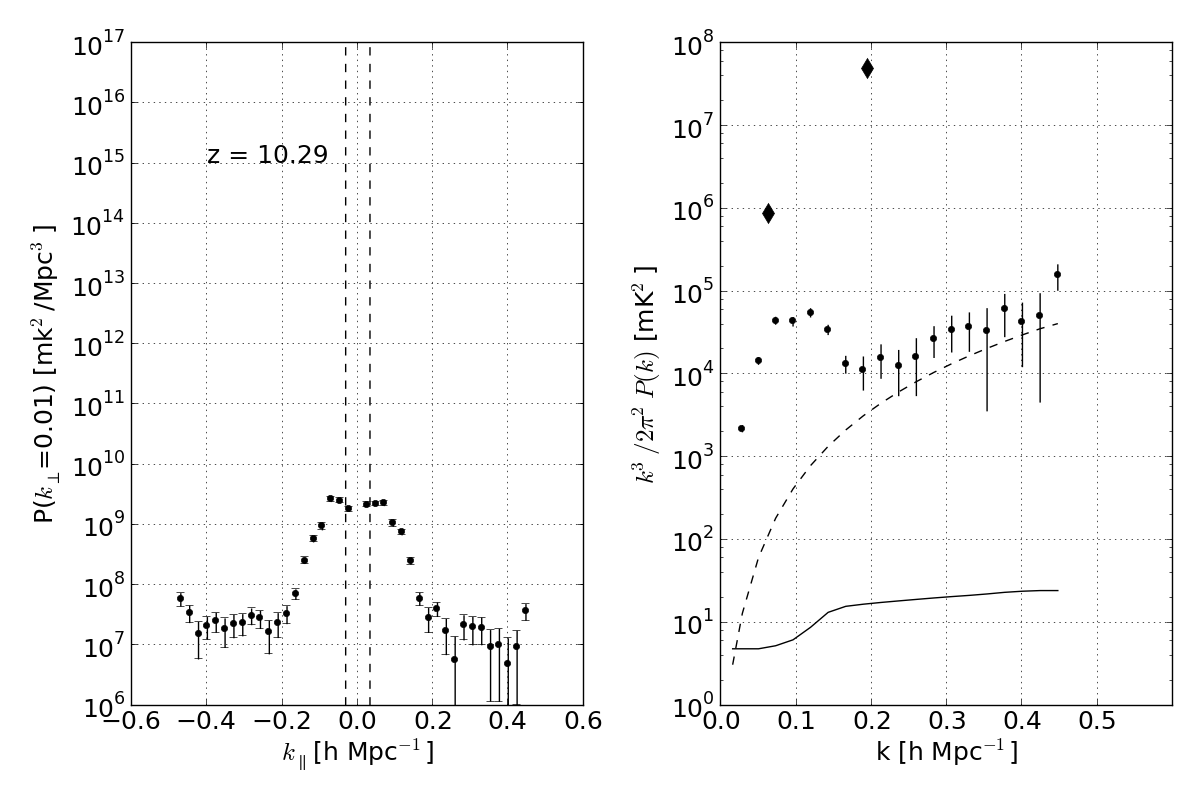
\includegraphics[width=0.45\textwidth]{{figures/pspec_log_z_10.29}.png}
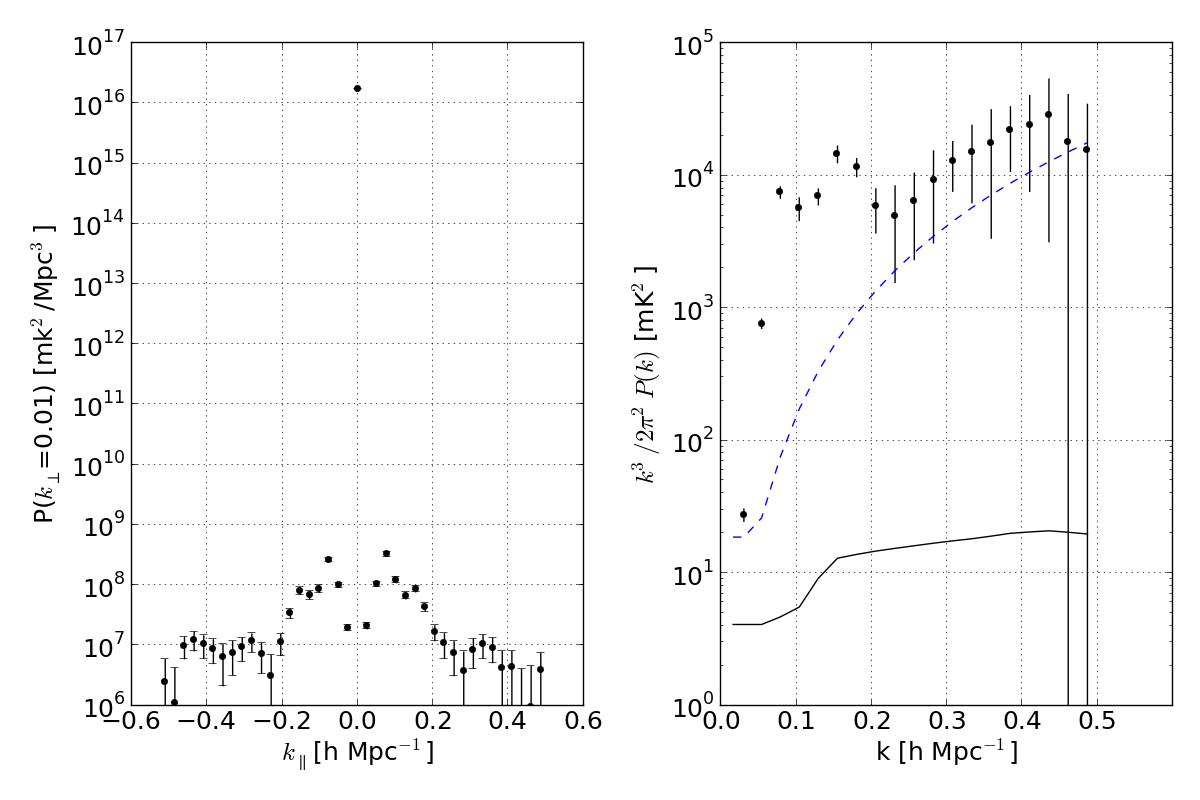
\includegraphics[width=0.45\textwidth]{{figures/pspec_log_z_8.54}.png}
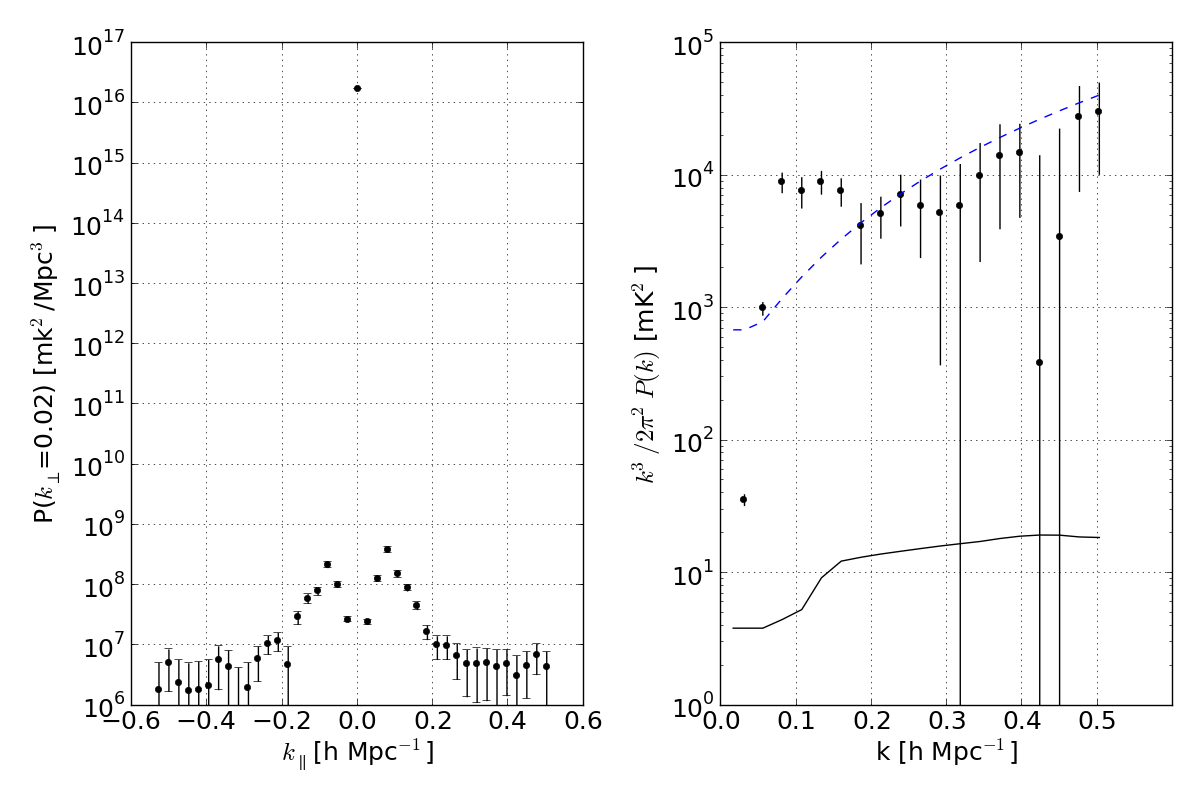
\includegraphics[width=0.45\textwidth]{{figures/pspec_log_z_7.94}.png}
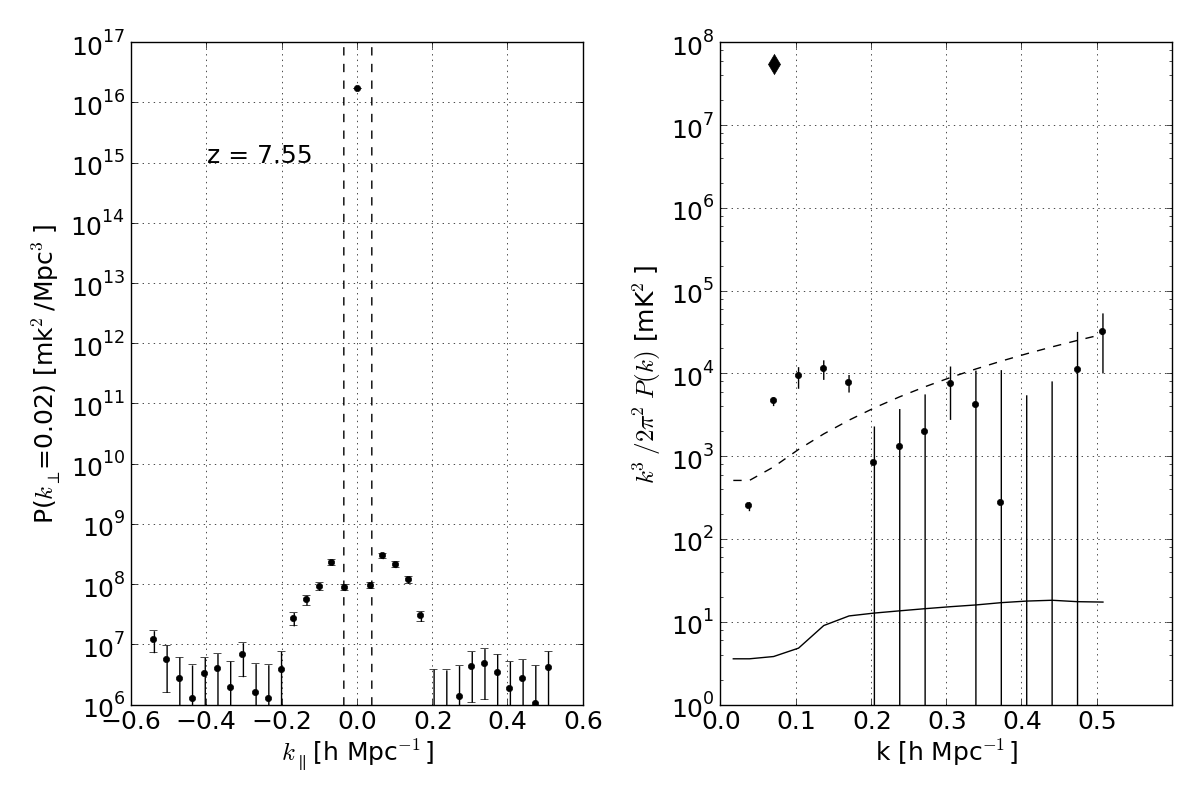
\includegraphics[width=0.45\textwidth]{{figures/pspec_log_z_7.55}.png}
\caption{\label{fig:pspecs} Left to right from top: power spectra centered on redshifts 10.3,8.5, 7.9, 7.68 and 7.6 (frequencies: 127, 149.5, 159.5 164.5, and 167 MHz.)  All with an effective bandwidth of $\pm$10MHz  covering the redshift span $\Delta z\approx$1421MHz ($B/f^2$) which ranges from 0.8 at $z=$10.3 to 0.45 at $z=$7.4.  The noise curve (blue dashes) is calculated using the method described in \cite{Pober:2014p10390}  and indicates the 1$\sigma$ confidence bounds on data points consisting purely of noise; 65\% of uncorrelated noise like data points will lie below the curve. However, note the caveats that due to the weighting of the delay transform, adjacent $k$ bins are 50\% correlated and that the sensitivity estimate is probably accurate to within a factor of two. The black line is a fiducial model at 50\% ionization \citep{Lidz:2008p8251}. . }

\end{figure}
\begin{figure}
\centering
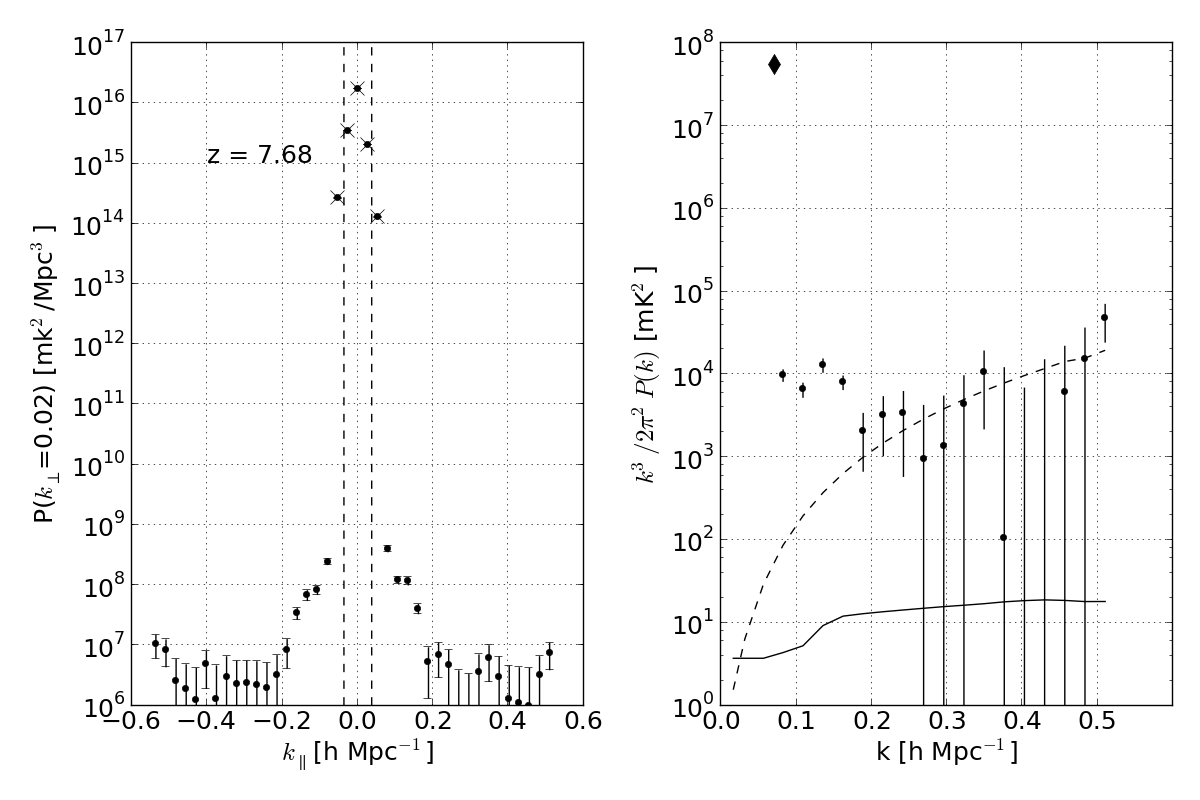
\includegraphics[width=0.45\textwidth]{{figures/pspec_log_z_7.68}.png}
\caption{\label{fig:P14compare} The redshift 7.68 bin has been reprocessed for comparison with the P14 result. Note that the LST range processed here is 3 hours less than P14 for a small reduction in sensitivity but large reduction in foreground }
\end{figure}


\section{Results}
\label{sec:results}
\subsection{Foreground Filtering and Noise Levels}
\label{sec:noise}
The root-mean-square of the residual measures how well we've removed foregrounds.  In Figure \ref{fig:noise} we examine $T_{rms}$ as calculated by differencing between adjacent channels and between redundant baselines. We see that in the last stage of coherent integration, the step between 40 second to 789 second integrations, the noise level decreases by the expected factor of $\sqrt{789/40}$.  At both stages the noise level found by both methods is roughly consistent with the theoretical level, only deviating significantly at the edges where the effective signal to noise due to the decreasing passband gain, Blackman Harris window, and uneven sampling (see Fig \ref{fig:bins}) drops precipitously. 

The theoretical visibility rms noise level is a straightforward calculation, but given the method employed here, should be given due description.
The noise level (eq \ref{eq:Trms}) is caused by the temperature of the sky (mostly due to galactic emission) which varies with LST and by the system noise, both on the scale of a few 100K. The noise of any long integration is also dependent on the number of observations in each LST.  The number of points in each bin is mostly determined by the observing schedule, which for PAPER is sunrise to sunset, but also by any flagging of data or observing outage (only 92 of the 103 days in the observing period have recorded data).  Unfortunately, technical problems limited the retention of the exact cumulative count of points averaged into each LST bin during the averaging process.  Here we have chosen to use the first order estimate based on the observing schedule to estimate the number of observations in each LST. Some bins are observed only a few times, while a slim range in the LST range 6 - 9 hours is observed on every night.  Over a number of lst bins $N_{lst}$ the average effective time per bin $N_{eff}$ is given by 

\[
\frac{1}{\sqrt{N_{eff}}} = \sum_\textrm{lst=1}^\textrm{lst=9}{\frac{N_{lst}}{\sqrt{N(lst)}}}
\]

On average each bin is in this dataset is effectively measured 39 times. Given this accounting of the number of samples $N(lst)$, we estimate the final rms temperature to be

\[
T_{rms}  = \frac{T_{sky}(lst) + T_{rcvr}}{\sqrt{2BtN(lst)}} \approx \frac{T_{sky} + T_{rcvr}}{\sqrt{2BtN_{eff}}}
\label{eq:Trms}
\]
where B and t are the 496kHz channel width and lst bin length, respectively. We model galactic temperature $T_{sky}$ by summing the \citep{deOliveiraCosta:2008p2242} global sky model  convolved by the PAPER beam as a function of lst averaged over the targeted lst range and $T_{rcvr}$=300K as the system temperature of 550K (found in P14) minus the mean galactic temperature from that time period (250K). The final result is plotted as a dotted line in Figure \ref{fig:noise} for before and after fringe rate filtering (t=40s and 789s)


The final fringe-rate step is the last coherent average of the processing routine and represents the last large gain in sensitivity; all following averaging steps are done incoherently on the square of the visibilities where sensitivity is gained at a much slower rate. For this reason the noise curves (bottom three curves of Figure \ref{fig:noise})  merit closer inspection.  At this sensitivity level we see a notable excess of power in the rms difference between baselines. Though the cause of this excess is unknown, it is suggestive of the excess covariance between redundant baselines which we remove in Section \ref{sec:power_spectrum} a hypothesis also supported by the high levels of residual foregrounds in the redshift 10.5 bin where the baseline difference rms is highest.




\subsection{Power Spectra}


In  Figure \ref{fig:pspecs} we show the  power spectra at different redshift bins --showing both the spherically averaged power spectrum plotted in $P_k$ units (left) and the final estimate of $\Delta^2$ -- and in Figure \ref{fig:slices} we see different $k$ mode slices as a function of redshift  all plotted with $2\sigma$ error bars.   The theoretical noise power spectrum is estimated using the method described in \cite{Pober:2014p10390} assuming a system temperature of 550K and the observing scheme described in Section \ref{sec:observations}.  Generally, both figures convey a picture of a power spectrum dominated by noise, with foregrounds encroaching from modes closest to the foreground contaminated modes.  Foreground dominance appears to grow with increasing redshift, mirroring the rise in baseline-to-baseline rms we found in Figure \ref{fig:noise}.  Recall that the wide-band foreground model we have subtracted is built by weighting the entire band by a Blackman-Harris window function.  This filter leads to the notch of missing power near $k_\parallel=0$  (except at z=7.68 where the foregrounds have been left in for comparison).  Only at redshift 10.3 is this notch nearly non-existent. Contributions to the foreground model from 126Mhz ($z=$10.3) are down-weighted by $\sim$75\%.  The $k=0.1$ slice (upper left of figure \ref{fig:slices}) is only a factor of $\sim$three away from the light travel horizon of $k=0.035$ and therefor most likely to be contaminated by low $k$ foregrounds. This $k$ mode is well above the noise and has a redshift  dependence  much the same shape as the $T_{rms}$ curve in Figure \ref{fig:noise}, with a minimum near redshift 8.5 and a dramatic rise above redshift 10.


%Across the entire band some $k$ modes appear to be dominated somewhat by non-noise systematics, these are not always clearly foregrounds because they appear at only certain $k$ modes rather than clearly emanating from small delays like in the z=10.3 power spectrum.  


%Possible assessment of comparison to noise.  Opt/Mid/Pes noise estimates.  If Opt noise => signal, if Pes=>systematics

\begin{figure}
\centering
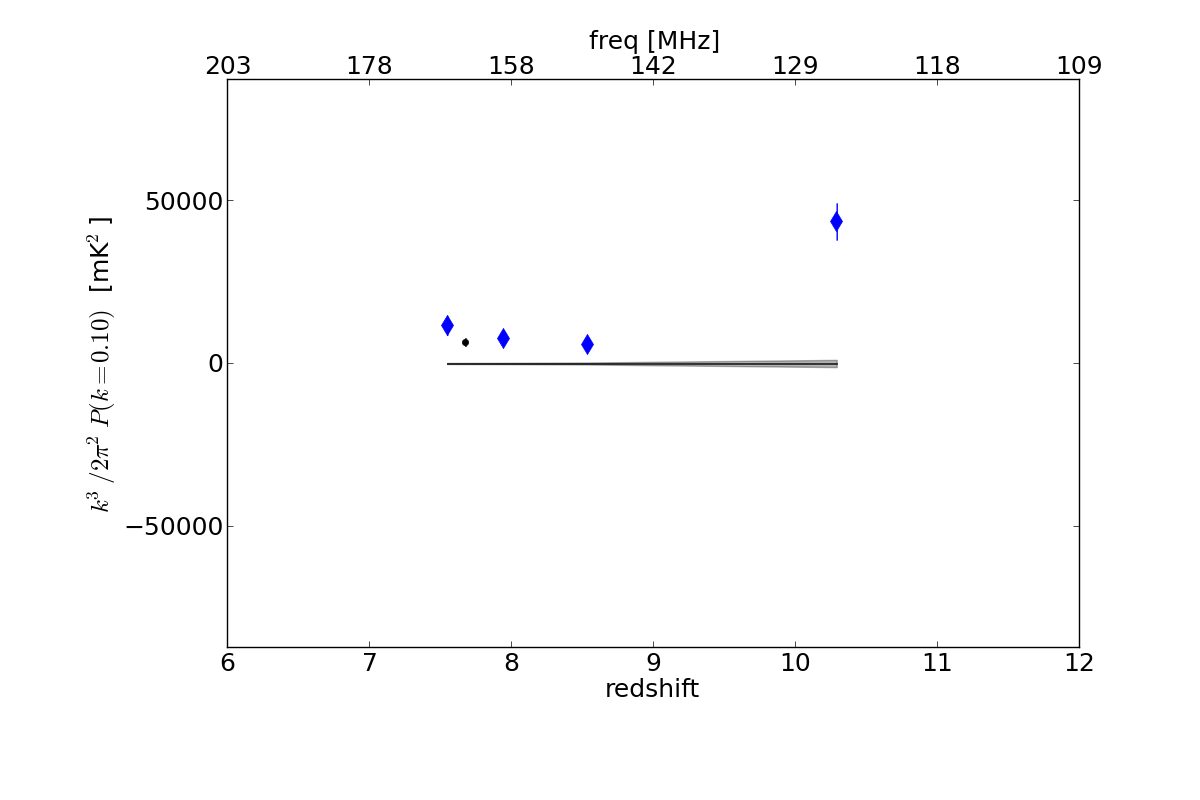
\includegraphics[width=0.48\textwidth]{{figures/psa32_pspec_k_0.10_lin}.png}
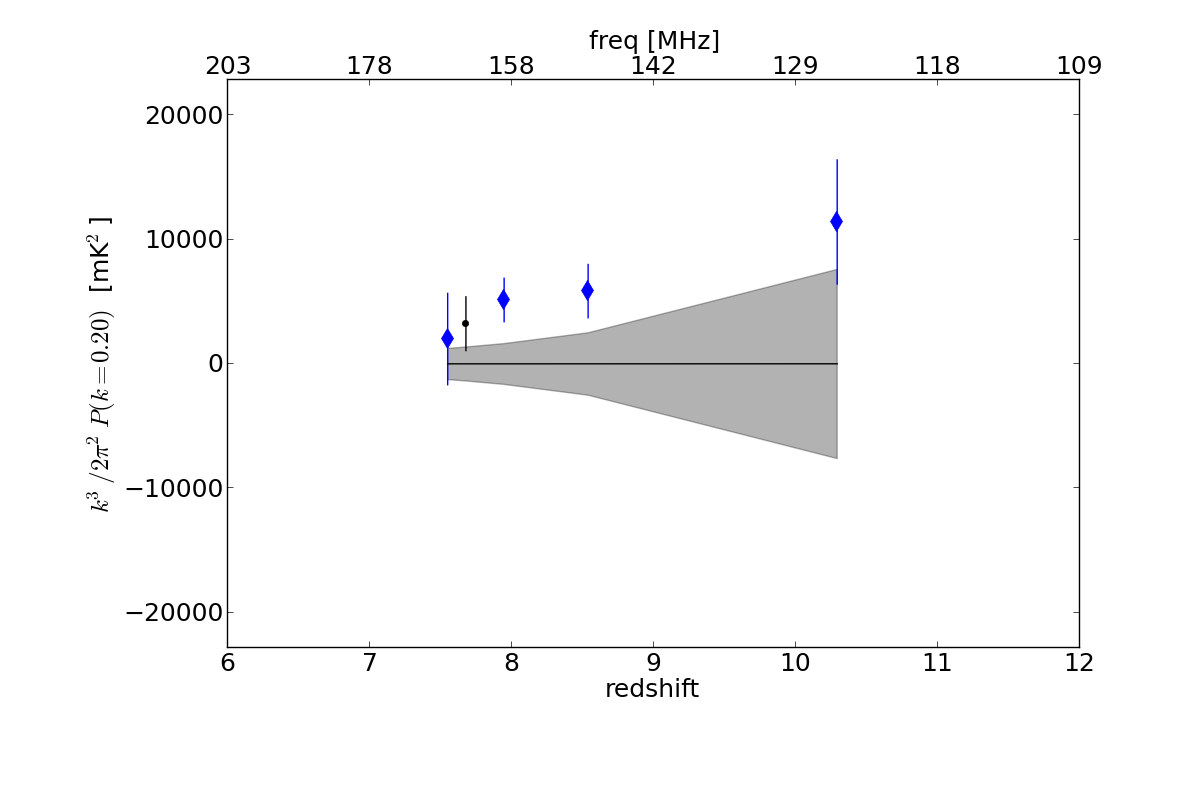
\includegraphics[width=0.48\textwidth]{{figures/psa32_pspec_k_0.20_lin}.png}
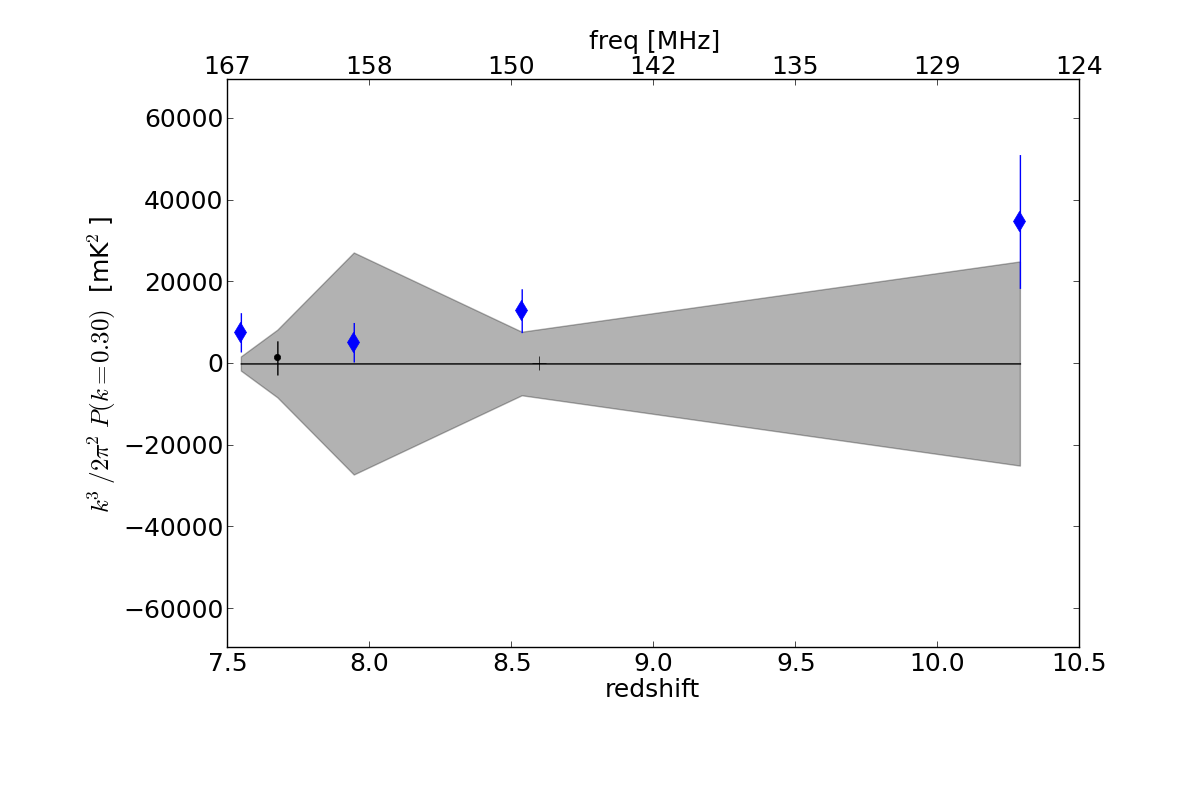
\includegraphics[width=0.48\textwidth]{{figures/psa32_pspec_k_0.30_lin}.png}
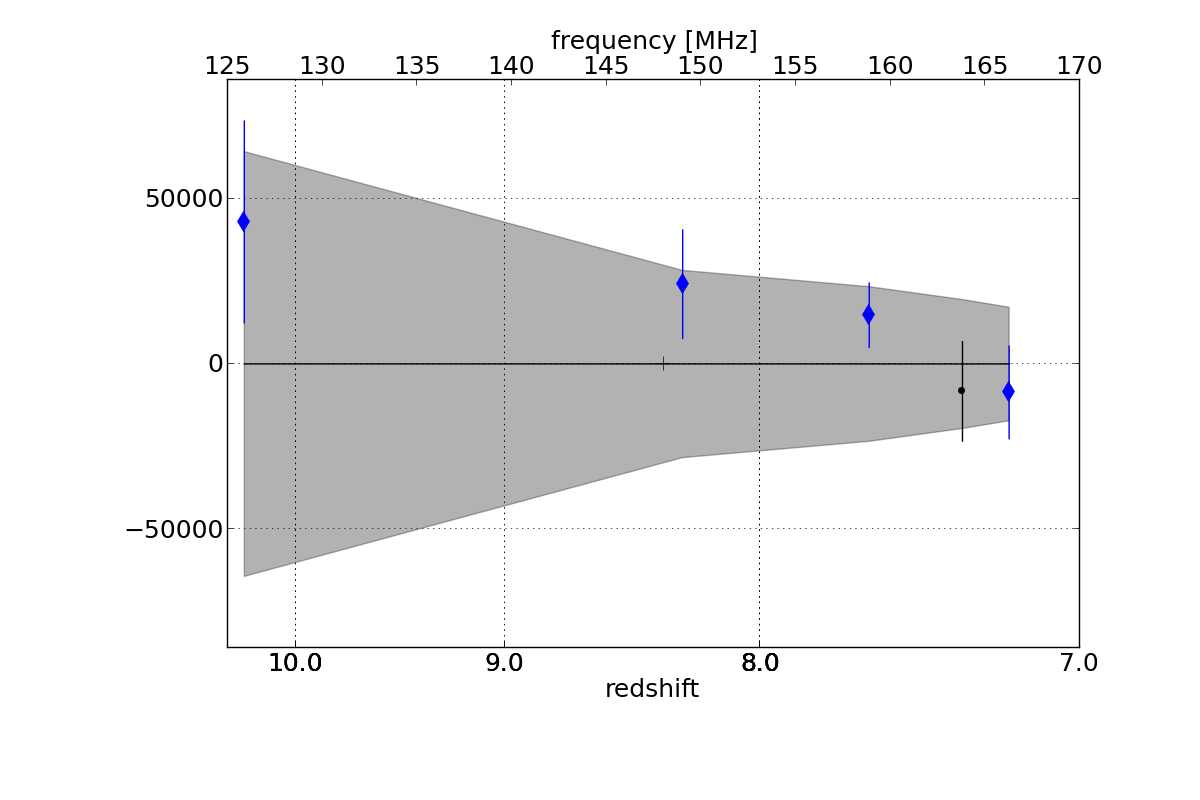
\includegraphics[width=0.48\textwidth]{{figures/psa32_pspec_k_0.40_lin}.png}
\caption{Power spectrum amplitude vs redshift at a selection of k modes. Left to right from top, k=0.1,0.2,0.3,0.4 hMpc$^{-1}$.  Parsons 2014 PAPER limit marked with thin black, this work marked with thick blue diamonds.  The k=0.1 hMpc$^{-1}$ bin (top-left), which samples the delay spectrum at only 2x the maximum horizon delay  is foreground dominated with  a redshift dependence similar to the  $T_{rms}$ residual in Figure \ref{fig:noise}.  The rest have amplitudes below the predicted noise level, but are not themselves perfectly consistent with noise, particularly at high redshifts. Though the points are all within the region predicted to be dominated by noise (grey) the variation between the redshifts and size of error bars suggests that a small residual signal is probably still present. The noise estimate incorporates a number of simplifications and could easily be off by a factor of 2-4.  \label{fig:slices}}
\end{figure}

%\subsection{Future Work}
%Further work is in progress to refine methods to include partially sampled data.

\section{Conclusions}
\label{sec:conclusion}



With this paper we have extended the redshift coverage of \cite{Parsons:2013p9876} to cover the range $10.3>z>7.6$.  Most of the power spectrum data points demonstrate a robust removal of foreground signals to the thermal noise limit, leaving systematics on the scale of the noise. Of particular note is the increased difficulty removing foregrounds at redshift 10.3.  This appears to be largely due to the centrally weighted Blackman-Harris filter used to provide a high dynamic range delay transform in the broadband foreground filter.  Future work will focus on more effectively removing foregrounds nearer to the edge of the band, opening more of the spectrum by being more tolerant of missing data, and better handling the removing of what residual foregrounds we do see with spectrum estimators which more robustly estimate power in the presence of residual foregrounds (e.g. \cite{Liu:2011p8763}).




%With only 32 antenna, this data lacks the sensitivity to exclude all but the most extreme models, however, it does demonstrate the ability of the wideband filtration method to affectively remove foregrounds to the precision needed to integrate a full season to the thermal noise limit.  As future observations with PAPER  will add sensitivity primarily by increasing to 128 antennae this projects well for our ability to reach design sensitivity.  The residual foregrounds analyzed here are all at or near the level of noise and expose the next level of removal required to access a wider redshift range. 





%\begin{align}
%\label{eq:BrightnessFluctuations}
% \Delta T &\approx \frac{T_S - T_{CMB}}{1 +z} \tau_{21} \nonumber\\
% &\approx T_0(z) \left( \frac{T_S - T_{CMB}}{T_S} \right) x_{HI} (1 + \delta) 
%\end{align}
%where $T_S$ is the 21cm line spin temperature, $x_{HI}$ is the local ionization fraction and $\delta$ is the mass over-density. All, save $T_0$, are position dependent.  $T_0$ encodes the global temperature evolution due to cosmological expansion
%\begin{align}
% T_0(z) & = 23~{\rm mK}~\left( \frac{\Omega_b h^2}{0.02} \right) \left[ \left(
% \frac{0.15}{\Omega_m h^2} \right) \left( \frac{1+z}{10} \right) \right]^{1/2}\nonumber\\
% & = 25~{\rm mK}~\left( \frac{1+z}{10} \right)^{1/2}
%\label{eq:Prefactor}
%\end{align}
%\citep[see, e.g., ][]{zaldarriaga_et_al2004,furlanetto_et_al2006}, where we have used the
%Planck 2013 parameters \citep{planck_et_al2013}.  



\bibliography{library}

\end{document}
